%************************************************
\chapter{Introduction}\label{ch:introduction}
%************************************************

Participatory sensing~\citep{Burke2006} is the process of leveraging user devices which are capable of various sensor measurements, to gather data in a bottom-up fashion and gain knowledge from the analysis of this data. 
It has already been applied in many varying domains, from traffic and transportation~\citep{Costa2012,Mathur2010}, environmental conditions~\citep{Hasenfratz2012,Mendez2011}, product pricing~\citep{Deng2009} to behavioural information~\citep{Miluzzo2008}.

In all of these applications, individual users or devices are gathering data which is then aggregated by a third party. Having collected this data, it is primarily this third party who reaps the benefits from the analysis of the data. The value of data gathered through these means has been estimated in the billions of dollars~\citep{Manyika2011}. While some organisations provide some return to contributors, usually in services, the equitability of this arrangement is debatable~\citep{VanDijck2009}. This has led to a call for the empowerment of users such that they can achieve a fair exchange for their data~\citep{BuckinghamShum2012}.

A key issue is the provision of tasks for participatory sensing. This is the process by which an entity determines a set of parameters to sense, and builds community and infrastructure for this purpose.
%(\citet{Burke2006} calls this user role \emph{initiator}). 
This is often a top-down process: of the applications we have mentioned the majority are centralised. This means that a single entity holds all of the collected data (often taking ownership or property rights of the data provided by others~\citep{ohara2010}), sets the policies regarding access to data and knowledge derived from the data, and controls how these policies are changed.

This approach is in direct contrast to how some of the most successful resources for data and knowledge have developed on the internet. 
The Open Data Institute has shown the benefits of open access to government data and that significant additional value can be generated by allowing others open and permissive access~\citep{Shadbolt2012}. 
Wikipedia\footnote{http://www.wikipedia.org} is an example where individuals contributing knowledge have created an encyclopedia at a scale which would be infeasible to do in a traditional top-down manner. 
Its continued success is down to its decentralised governance which allows its users to direct the trajectory of site policy~\citep{Famiglietti2011}.

To understand the implications of how these organisational structures affect user participation and the associated benefits from the data and knowledge generated, we look at how social organisations have developed around knowledge repositories.
\citet{Ostrom2003} argue that information can be seen at a common-pool resource and thus analysed using the considerable existing literature on the commons~\citep{Hess2007}. 
Some initial investigations have been applying this approach to user-generated content~\citep{Pitt2012} which we take further here.

From her significant field work on physical commons, \citet[p.42]{Ostrom1990} outlined `the problem of supplying a new set of institutions'. 
This is the problem that in order to form an organisation someone must first provide an initial set of rules by which the organisation and its members are governed.
This is a difficult task as there are many stakeholders to satisfy under changeable conditions. Through survey of both successful and unsuccessful institutions Ostrom extracted a set of principles which were more prevalent in successful cases.

In participatory sensing we can empower users by providing them with the ability to supply institutions, and the knowledge to assess the effect of the rules and organisational structure governing sensing applications. 
We review the literature analysing knowledge commons to derive an analytic framework for institutional design of participatory sensing applications construed as a provision and appropriation system.  %This will then allow us to understand how we can provide an organisation for the management of data and knowledge for participatory sensing.
We can then derive guidelines for firstly how a self-organising participatory sensing application can function as a provision and appropriation system using a knowledge commons, and secondly how such a system can be supplied.

%Propositions/contributions:
%\begin{itemize}
%\item That participatory sensing can be seen as an information and knowledge commons and thus characterised as a provision and appropriation system.
%\item That such a system for participatory system can adhere to Ostrom's principles for enduring institutions.
%\item We can formalise this system to allow autonomous, heterogeneous agents to provision, participate in and modify an electronic institution for the management of information and knowledge resources for participatory sensing in a sustainable and equitable way.
%\end{itemize}

This paper is organised as follows: In Section~\ref{sec:commons} we introduce the theory behind information and knowledge as a commons, and how participatory sensing can be seen as such a commons. 
We then review participatory sensing applications in Section~\ref{sec:review}. This is followed by an analysis of participatory sensing as a knowledge commons according to Ostrom's institutional analysis and development framework in Section~\ref{sec:iad}. 
This analysis allows us to then create a formal representation of a system for self-organising management of a participatory sensing application as an information and knowledge commons and subsequently evaluate this system. 
Our evaluation shows that such institutions could enable autonomous, heterogeneous agents to manage information and knowledge commons used for participatory sensing applications while maintaining important criteria such as sustainability, participation standards and equity.

We finish, in Section~\ref{sec:conclude}, with some conclusions derived from this critical review and analysis of
some representative participatory applications,
in particular that:
\begin{itemize}
\item Data clouds in open participatory sensing applications can be construed as information and knowledge commons and thus characterised by provision and appropriation actions; and
\item A system for access control (i.e. provision and appropriation) in participatory sensing applications can be designed according to Ostrom's institutional design principles for self-governing institutions and formally specified in an action language.
%\item That such institutions can enable autonomous, heterogeneous agents to manage information and knowledge commons used for participatory sensing applications while maintaining important criteria such as sustainability, participation standards and equity.
\end{itemize}

This provides the foundations for engineering knowledge commons for the next generation
of participatory sensing applications, in which the data generators are also the primary beneficiaries.

\section{Preliminary Definitions and Assumptions}

\subsection{Multi-agent systems \& Intelligent Agents}\label{sec:agents}

The term \ac{MAS} is a broad term encompassing an array of different concepts and applications. While the meaning of the term can be decomposed to be a system of multiple agents, the definition of an agent remains to be settled~\citep{Wooldridge2002}. There is some consensus that, firstly agents are computer systems situated in an environment, and that they are autonomous. Other important features of agency are given as~\citep{Wooldridge1995,HayesRoth1995}:
\begin{itemize}
\item \emph{reactivity}---agents perceive their environment, including other agents, and react to changes in it.
\item \emph{proactivity}---agents are able to exhibit goal-directed behaviour.
\item \emph{communication}---agents can have some kind of social capacity to interact with other agents.
\end{itemize}

Thus the requirements for agency are tied to both the capabilities of system, and the way in which it makes decisions (in contrast to agency in social sciences which only requires autonomy). These requirements act as a way of excluding basic systems, such that not all systems and programs would be classified as agents~\citep{Franklin1997}.

When in an environment, an agent reads the state of the environment via sensors, and performs actions to change the state of the environment. In most cases the control that the agent can exert on the environment will only be partial, in that it can influence the state of the environment. The effect of an action may not be deterministic, or it may not have any affect at all, depending on the properties of the environment~\citep{Wooldridge2002}.

The properties of an environment can be classified according to several relevant criteria~\citep[p.46]{Russell2003}:
\begin{itemize}
\item \emph{Accessible}---If an agent can perceive the complete environment state via its sensors, then the environment is accessible to this agent.
\item \emph{Deterministic}---If the next state of the environment is determined purely from the current state and actions of agents, then it is deterministic.
\item \emph{Episodic}---In an episodic environment the quality of actions do not depend on previous actions.
\item \emph{Static} or \emph{dynamic}---If the environment can change while an agent is deciding on an action then the environment is dynamic for the agent; otherwise it is static.
\item \emph{Discrete} or \emph{continuous}---If the set of possible environment states is finite, then the environment is discrete; otherwise it is continuous.
\end{itemize}

\citet[pp.31--32]{Wooldridge2002} provides a formalisation of an abstract \ac{MAS}. This defines a \emph{run} of an agent in an environment as a sequence of interleaved environment states and actions, representing the history for that agent; a \emph{state transformer} function which defines the effect that agents actions have on the environment state; and an \emph{agent function} which maps a \emph{run} for an agent to an action, representing an agent's decision process.

\section{Methodology}

In this thesis we follow closely a methodology called \ac{SIC}~\citep{Jones2013}. This is a method for the design of socio-technical systems from the analysis of social and organisational concepts. Built upon the synthetic method underlying research in artificial societies and artificial life~\citep{Steels1994}, the formalisation of social relations in multi-agent systems~\citep{Neville2004}, and other attempts to apply ideas from the social sciences to the design of computational systems~\citep{Edmonds2005}, it provides a series of steps to go from an observed social phenomenon to an observed performance of a derived computer model under controlled experimentation conditions. These steps are illustrated in \autoref{fig:sic}.

\begin{figure}
\caption[Methodology for sociologically inspired computing.]{Methodology for sociologically inspired computing~\citep{Jones2013}.}\label{fig:sic}
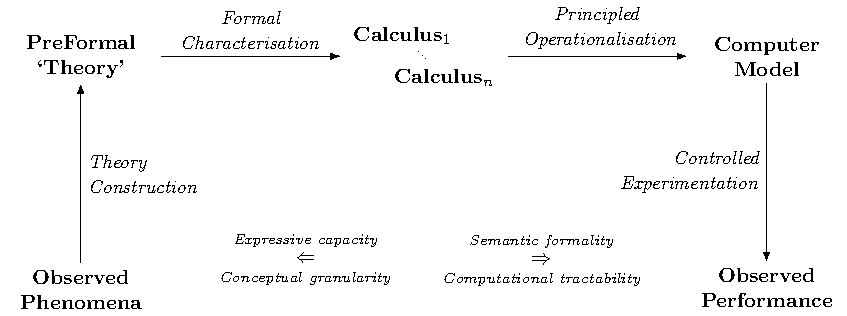
\includegraphics[width=\linewidth]{gfx/sic}
\end{figure}

% TODO Interleave what we actually do.
We begin with an observed phenomenon, for example, from the social sciences, a human social, legal, or organisational system. The process of \emph{Theory Construction} generates a \emph{PreFormal Theory}, usually expressed in a natural language. \emph{Formal Characterisation} creates a specification of this theory in a calculus of some kind, where `calculus' is meant to be any system of calculation or computation based on the manipulation of symbolic representations. This calculus is then embedded in a computer model in the \emph{Principled Operationalisation} step. This computer model enables simulations that can include both implementations of individual agents, and/or treatment of large populations. Through \emph{Controlled Experimentation} with this computer model we can observe the performance of the model.

Through our use of this methodology we have two major contributions to the \emph{Principled Operationalisation} and \emph{Controlled Experimentation} steps. The platform Presage2~\citep{Macbeth2014} which enables both of these steps, and a rule engine for Electronic Institution which enables rapid operationalisation of common concepts from Electronic Institutions, with flexibility to accommodate further rules from the calculus. These contributions are presented in \autoref{ch:presage} and \autoref{ch:droolseinst} respectively.
